\documentclass[titlepage]{article}
\usepackage[T1]{fontenc}
\usepackage[utf8x]{inputenc}
\usepackage{placeins}
\usepackage{graphicx}
\usepackage[english]{babel}


\author{Luca Massini \and Daniele Nicolò}

\title{Design Document
\\  Safestreets}

\date{release date to be defined}
\begin{document}
\maketitle
\newpage 
\tableofcontents
\newpage
\section{Introduction}
\subsection{Purpose}
	This document is necessary to describe the architecture of the system from several points of view. An architecture can be expressed in terms of the system components and their interactions with each other.\\
	An architecture can be thought as a starting point for possible future changes,according to the needs of the stakeholders.\\
	Finally the requirements mentioned in the RASD document will be explained here from an architectural perspective, that can be seen with component, deployment and runtime views. 
\subsection{Scope}
Safestreets is a service that allows private users to inform authorities about parking and traffic violations. A user must take a picture of the violation and describe it and the place where it occurred. An image recognition algorithm is run on the sent picture. A user has also the possibility to see the safety of the streets and the parking areas and to check the most reported streets and vehicles. \\
The system offers also the possibility to receive suggestions in order to improve the streets safety. This feature is available only for municipality accounts. These  suggestions are generated by the system using an algorithm that retrieves the information from the users' reports and also from the data given by the municipality.
\subsection{Definitions,Acronyms and Abbreviations}
\subsubsection{Definitions}
TODO
\subsubsection{Acronyms}
TODO
\subsubsection{Abbreviations}
TODO
\subsection{Revision History}
TODO
\subsection{Reference Documents}
TODO
\subsection{Document Structure}
The following sections are structured as below:
\begin{itemize}
	\item \textbf{Architectural Design: }In this section there will be the description of the system from the architectural point of view. This means to show the components and their interactions with each other and to explain the design patterns choices and the architectural styles. 
	\item \textbf{User Interface Design:} In this section there is an explanation,in terms of user experience (UX), of the user interfaces already showed in the RASD mockups.
	\item \textbf{Requirements Traceability:} Here we describe how the requirements already explained in the RASD match with the design choices done in this document.
	\item \textbf{Implementation, Integration and Test plan:} Here there is the description of how we will implement all the components, how we will integrate them together and finally how we will test both the single components and also the integrated system.
	\item \textbf{Effort spent:} Here there is the division of the work hours of each member of the group and the description of the tasks completed and related time spent.
\end{itemize}
\begin{figure}[h]
\section{Architectural Design}
	\subsection{Overview}
In the figure below it is shown the architecture of the entire system. This description has to be intended only as an overview and because of this some details are not shown.
	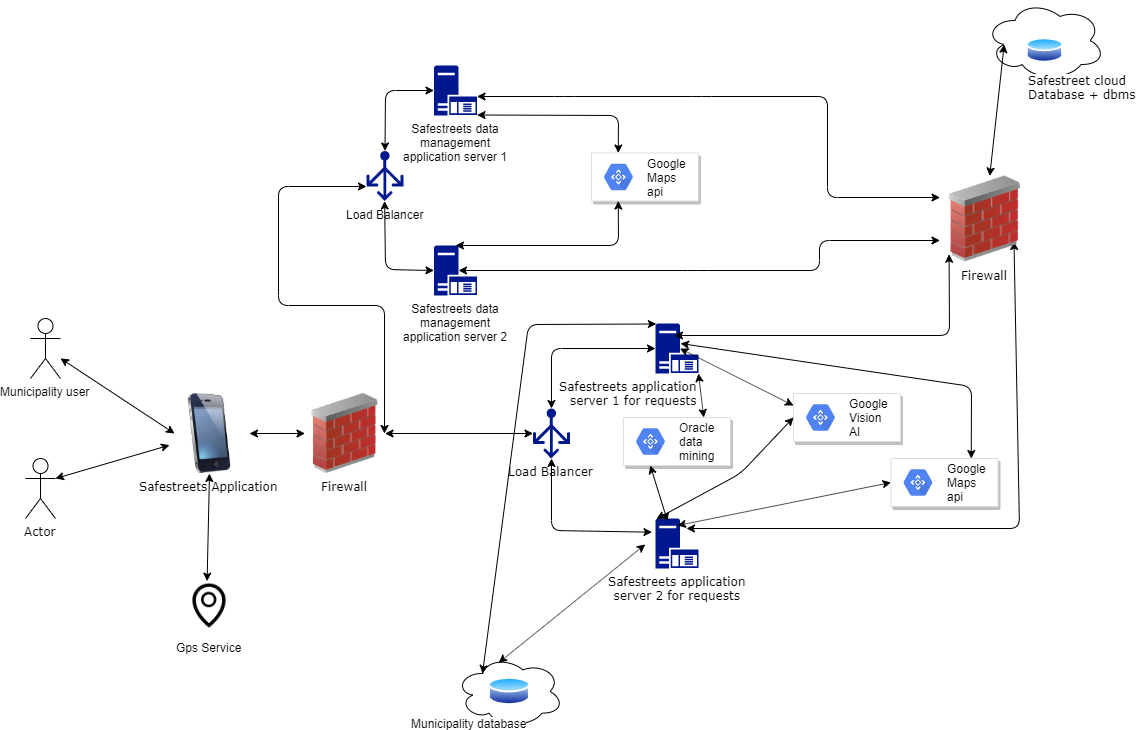
\includegraphics[scale=0.465]{Diagrams/overview.png}
	\caption{Architectural overview}
\end{figure}
\FloatBarrier

In this system we have two clusters of servers and two types of servers. One is specialized in taking the requests that comes from outside the network whereas the other one is specialized in managing the reports that come from the private users. Obviously it is necessary to define what we mean by request and reports.In this case a report for us is a report of a violation sent via smartphone application to the system. Instead, a request is any possible thing that the the private user/municipality user can ask to the system to do. Obviously a request cannot be a violation report and the other way around.\\
 The load of requests is managed by the load balancer in order to guarantee a balanced load. The balanced load can be translated then in a better efficiency in the service. In fact thanks to duplication of components it is possible to satisfy requests in parallel and so faster. The redundancy of resources can make the system more fault tolerant.\\
 Both the clusters communicate to the database of the application. In particular the servers devoted to requests interact also with the database of the municipality to have information about the accidents. Thanks to the interaction with the municipality database it is possible to have more detailed information about the safety.\\
The storage is managed with a cloud computing approach in both the databases. Thanks to this type of approach it is possible to reduce or increase resources according to the number of requests in a specific moment. This is very important in order guarantee elasticity in the resources devoted to the service.\\ 
\subsection{Component view}
Here there is the description of the software components that will be implemented in the specific hardware.

\begin{figure}[h]
	\subsection{Deployment view}
	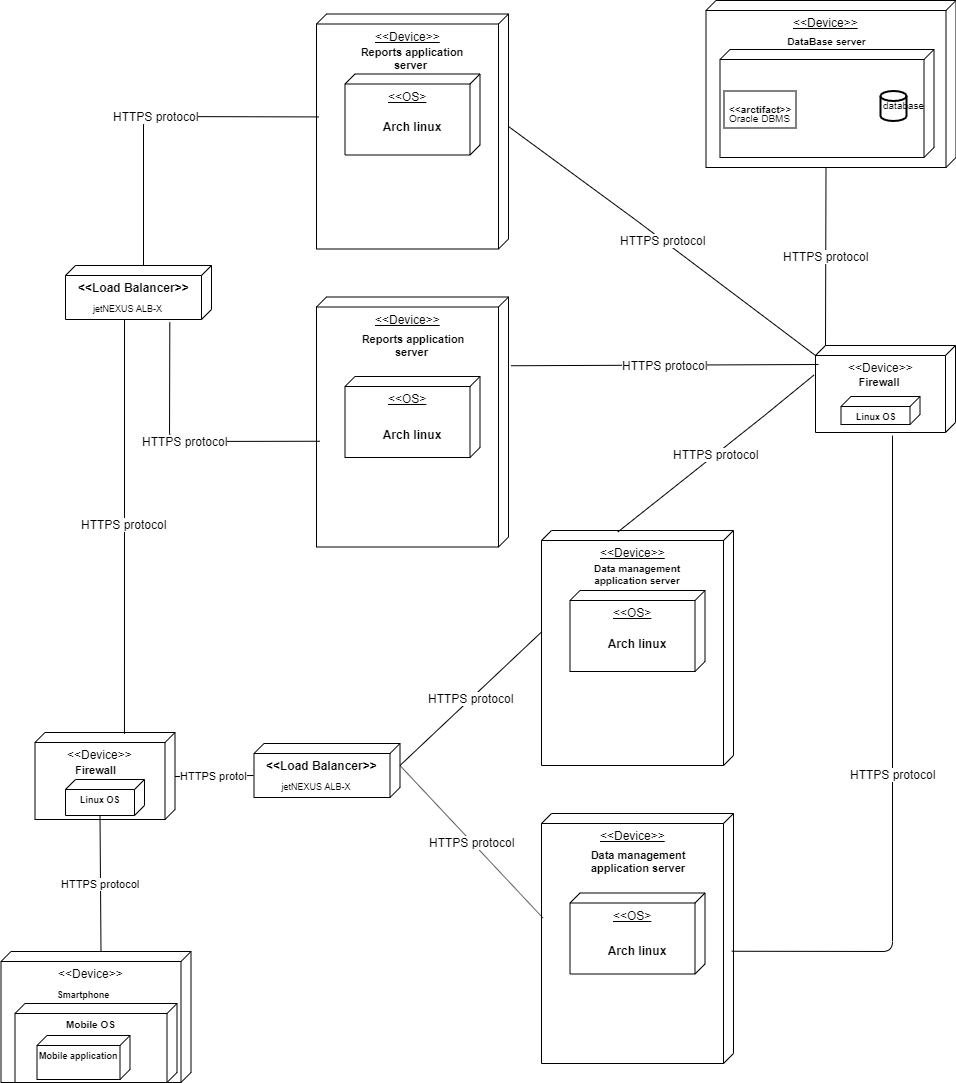
\includegraphics[scale=0.465]{Diagrams/Deployment diagram.png}
	\caption{Deployment diagram}
\end{figure}
\FloatBarrier

This diagram is very similar to the one in the overview. It express some aspects which have been already explained and some others are explained only here. In fact we can see all the operating systems for each server and also the protocol used in the communication between the devices.
Here you can find a brief description of what the single components do:
\begin{itemize}
\item \textbf{Firewall:} Firewalls are well known for sure by the majority of the people but we think that it is important to describe their operation the same. Firewalls are placed between the internal network and the external ones.They are used to filter the incoming/outcoming packet traffic. Through a set of rules they decide if a packet can pass or (unique alternative) be blocked.  This can be very useful to guarantee a better system safety.
\item \textbf{Load Balancer:} Load Balancers are used to improve the workloads across multiple computing resources. Thanks to load balancer the load can be balanced in an optimal way.This can make the system more performing and can also improve the fault tolerance of the system because of redundancy.
\item \textbf{Servers:} In this architecture we can find two clusters, each one containing 2 application servers. The servers are specialized with no overlap of functionalities. One is specialized in the managing of the reports by the private users. It must update the database with the new incoming data only after having done all the checks about the validity and correctness of the report.\\
The other server deals with the managing of the requests by the private users or municipalities. It is in charge of check the correctness and validity of the request,and then it must run all the data mining algorithms necessary to retrieve the result and finally send the results to the right private user.
\item \textbf{Databases:} The databases are cloud databases managed thanks to an API that will be provided by the provider of the service. We have only one cloud database used to store all the Safestreets data. Another cloud database is the external one of the municipality. Safestreets has only a special view of the part of the municipality database concerning the accidents. The access to the external database will have to be possible thanks to an API provided by the municipality. This API will have to follow a standard provided by us.
\end{itemize}
\subsection{Runtime View}
\subsection{Component interfaces}
\subsection{Selected architectural styles and patterns}
\subsection{Other design decisions}

\begin{figure}[h]
	\section{User interface design}
Here there will be shown the user interfaces with the help of UX diagrams. In particular there is shown the flow that the user will follow to navigate inside the application.Some aspects concerning the user interfaces design have been already treated in the "Requirement Analysis and Specification Document",if the reader wants to understand in a better and more detailed way, he/she is strongly suggested to refer also to it.
UX diagrams:\\
	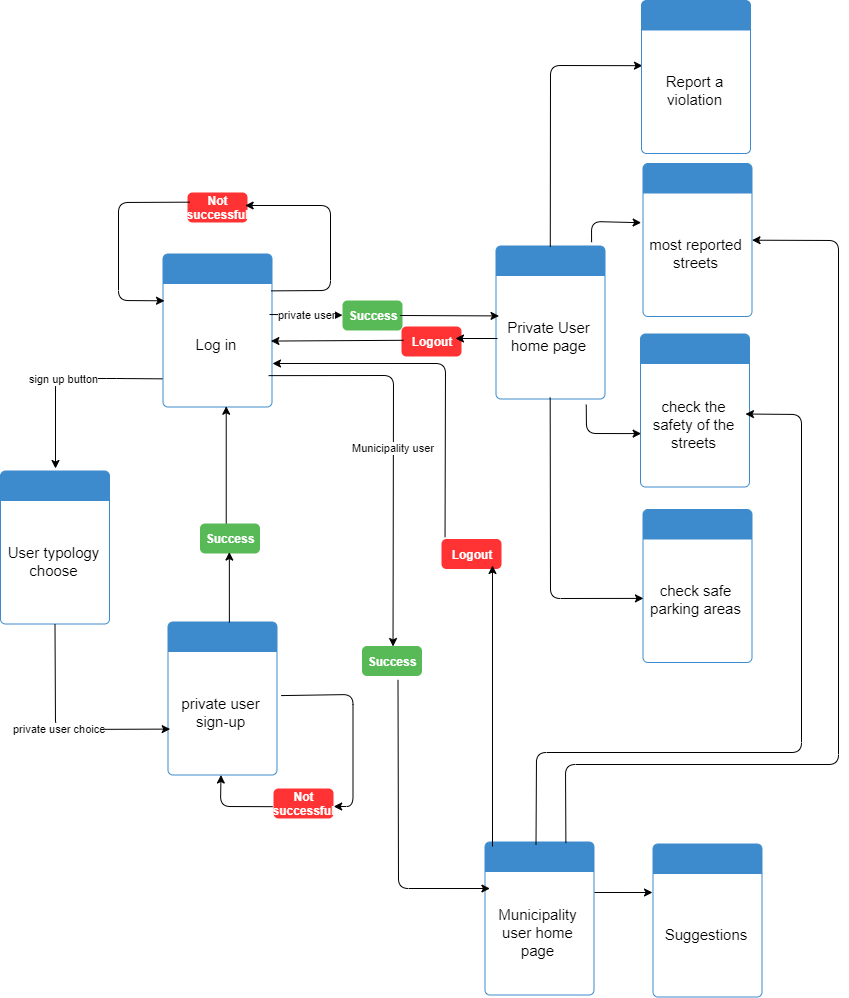
\includegraphics[scale=0.48]{Diagrams/UX diagram.png}
	\caption{UX diagram}
\end{figure}
\FloatBarrier



\end{document}